\section[Theorie]{Theorie \textnormal{\cite{faraday}}}
\label{sec:theorie}

\subsection{Bandstruktur}

\begin{figure}
    \centering
    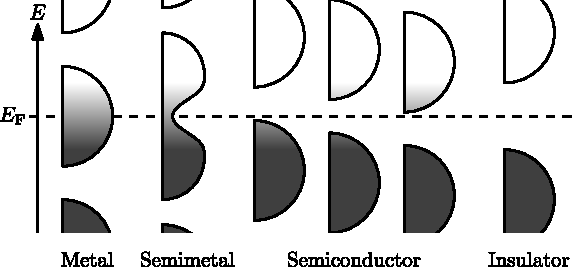
\includegraphics[width=0.8\textwidth]{content/grafik/bandstructure.pdf}
    \caption{Energieschemata verschiedener Materialklassen im Vergleich. \cite{wiki_band}}
    \label{fig:baender}
\end{figure}

\begin{figure}
    \centering
    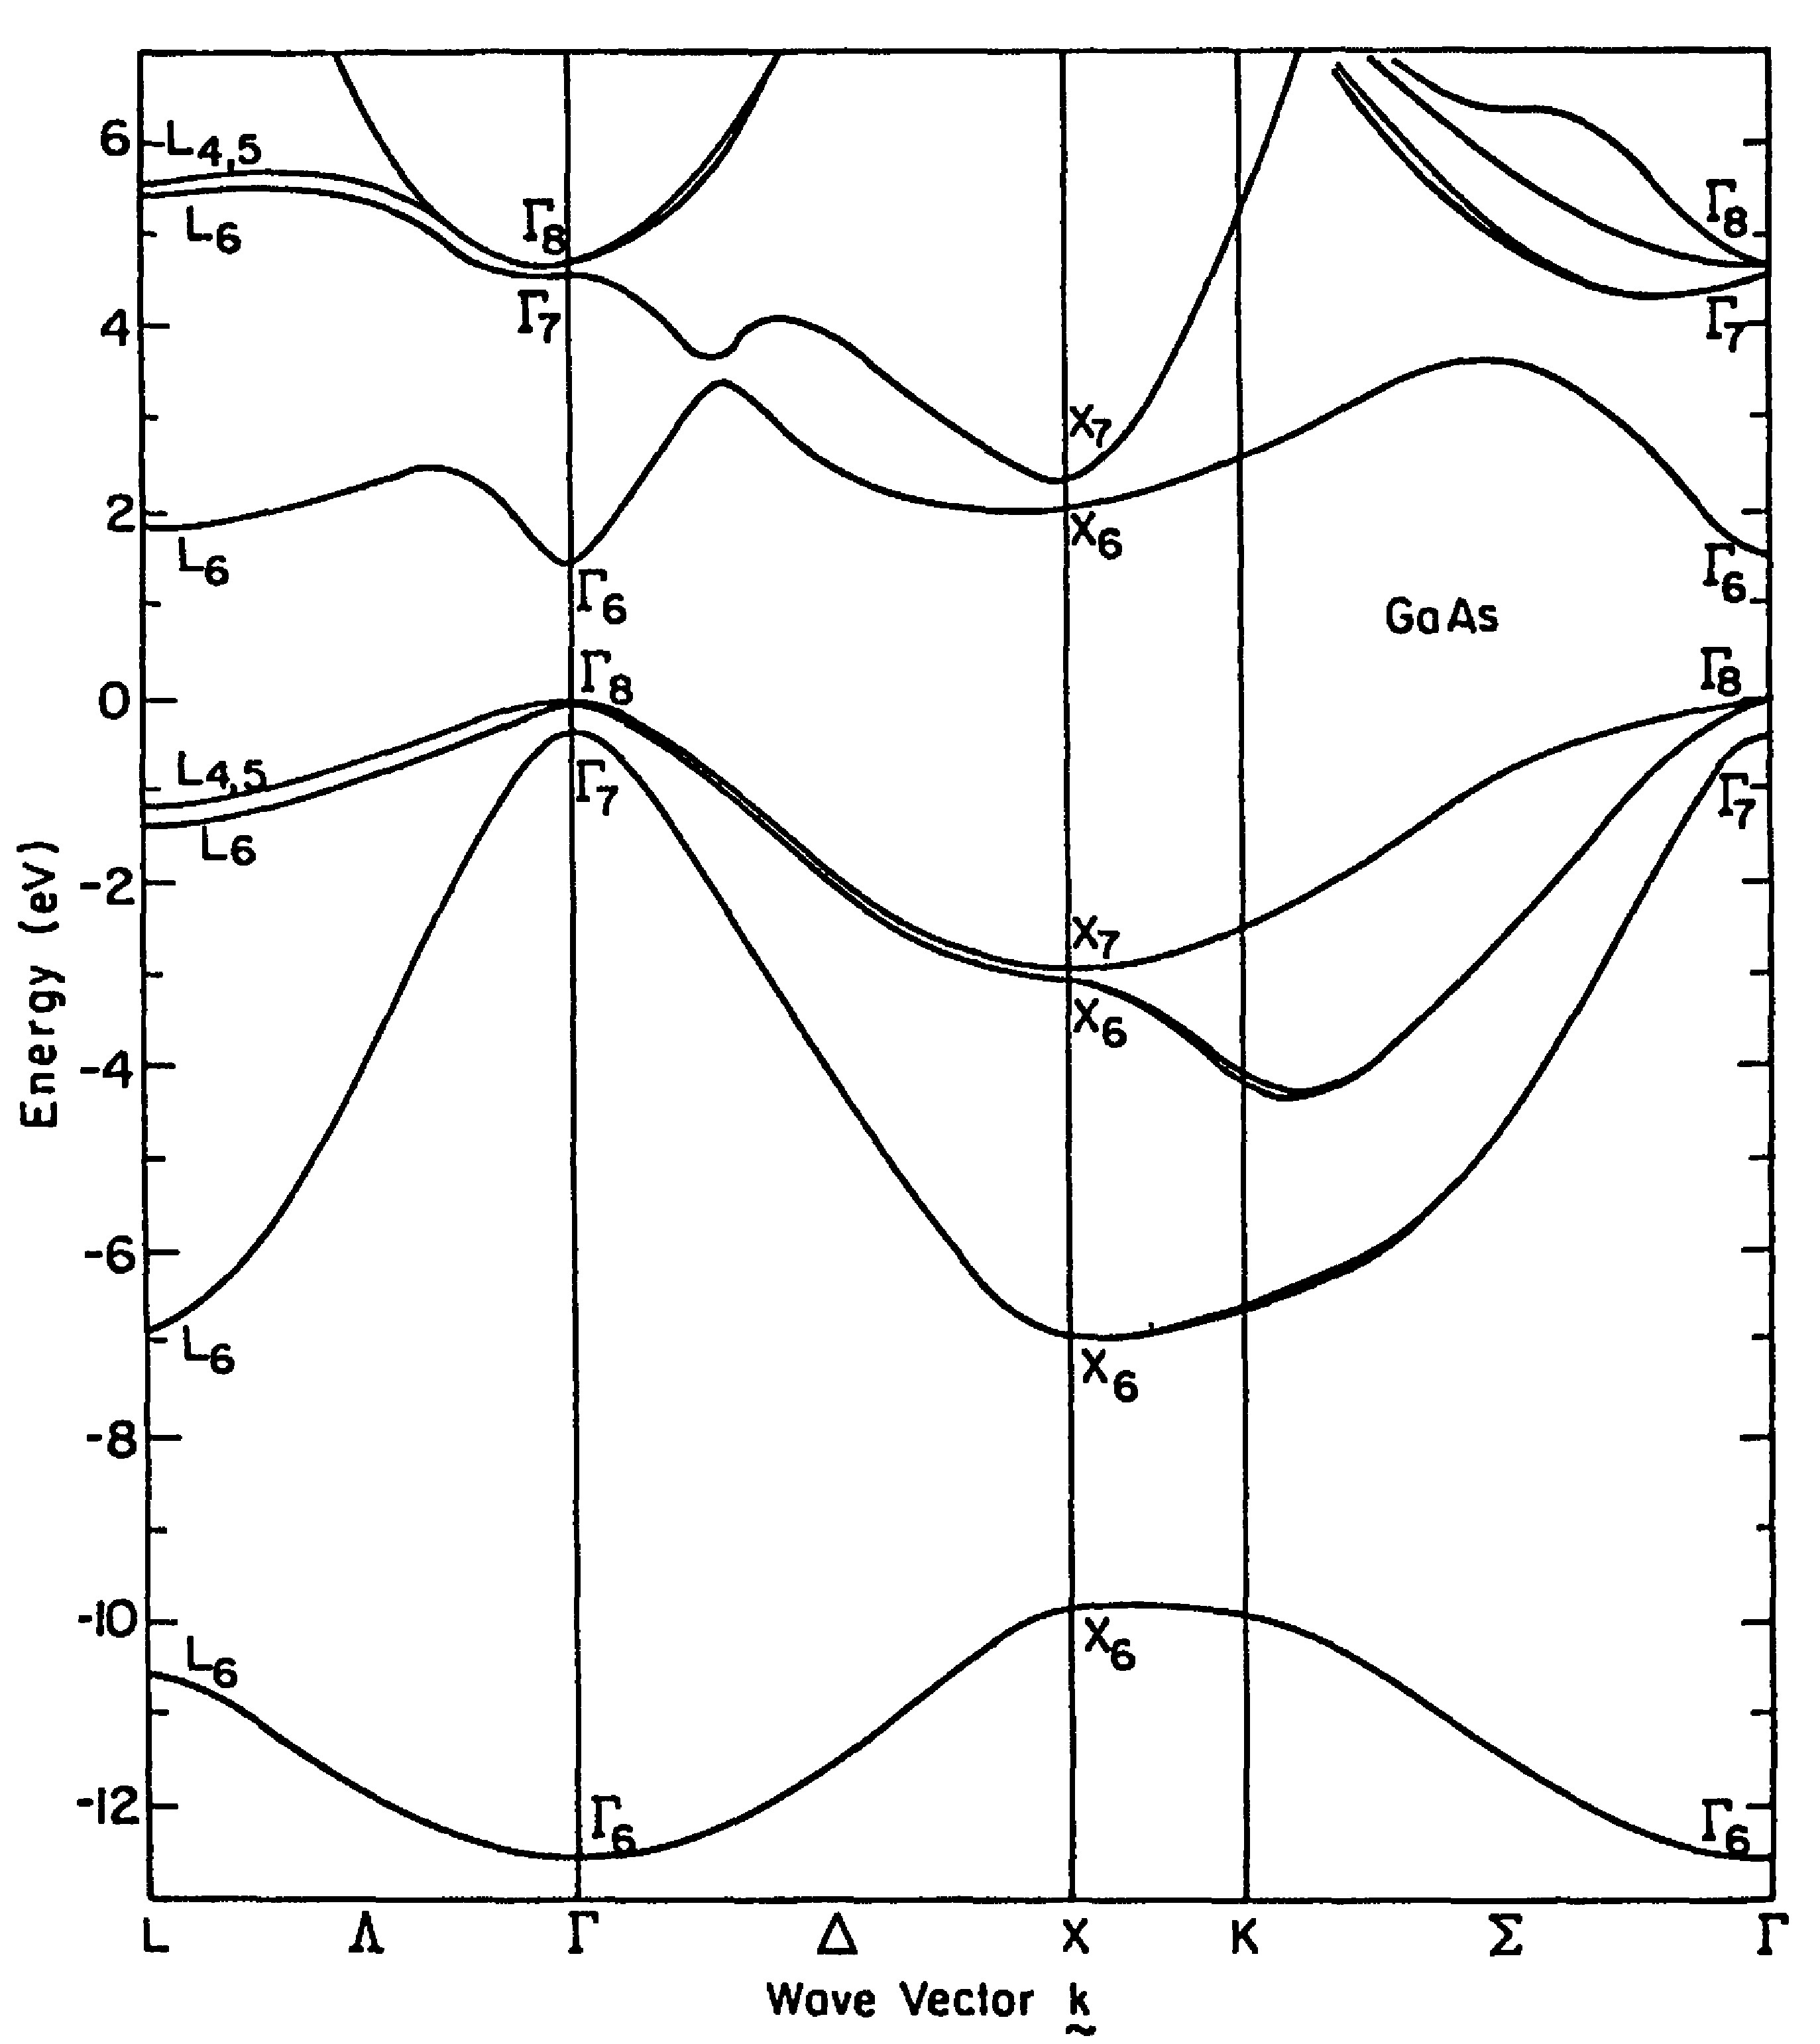
\includegraphics[width=0.6\textwidth]{content/grafik/bandstruktur.jpg}
    \caption{Berechnete Bandstruktur von GaAs um die Bandlücke. \cite{coh_jam_el}}
    \label{fig:band}
\end{figure}

\subsection{Dotierung}

\subsection{Faraday-Effekt}

\begin{figure}
    \centering
    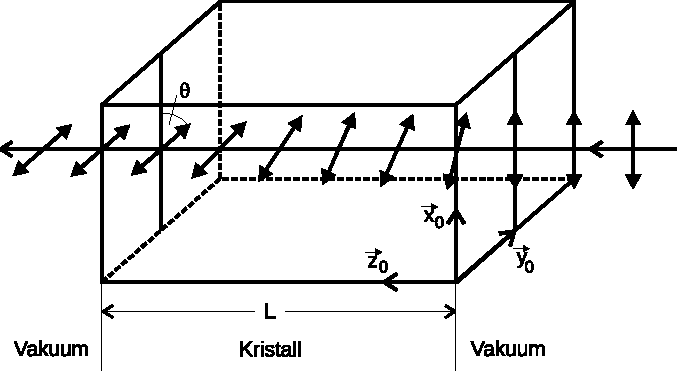
\includegraphics[width=0.7\textwidth]{content/grafik/drehung.pdf}
    \caption{Drehung der Polarisationsebene einer Lichtwelle beim Durchgang durch einen Kristall. \cite{faraday}}
    \label{fig:drehung}
\end{figure}

\begin{align}
    \bm{E}(z) = \pfrac{1}{2} \left(\bm{E}_R(z) + \bm{E}_L(z)\right)
\end{align}

\begin{align}
    \bm{E}_R(z) &= E_0 \left(\bm{\hat{x}} - i \bm{\hat{y}}\right) e^{ik_Rz} \\
    \bm{E}_L(z) &= E_0 \left(\bm{\hat{x}} + i \bm{\hat{y}}\right) e^{ik_Lz}
\end{align}

\begin{align}
    \bm{E}(0) = E_0 \bm{\hat{x}}
\end{align}

\begin{align}
    \bm{E}(L) = \pfrac{1}{2} E_0 \left( 
                \left( e^{ik_RL} + e^{ik_LL} \right) \bm{\hat{x}} +
                \left( e^{ik_RL} - e^{ik_LL} \right) \bm{\hat{y}} \right)
\end{align}

\begin{align}
    \psi &\equiv \pfrac{L}{2} (k_R + k_L) \\
    \theta &\equiv \pfrac{L}{2} (k_R - k_L)
\end{align}

\begin{align}
    \bm{E}(L) = \pfrac{1}{2} E_0 \left( 
                \left( e^{i\psi}e^{i\theta} + e^{i\psi}e^{-i\theta} \right) \bm{\hat{x}} +
                \left( e^{i\psi}e^{i\theta} - e^{i\psi}e^{-i\theta} \right) \bm{\hat{y}} \right)
\end{align}

\begin{align}
    \bm{E}(L) = E_0 e^{i\psi} (\cos\theta \,\bm{\hat{x}} + \sin\theta \,\bm{\hat{y}})
\end{align}

\begin{align}
    v = \pfrac{\omega}{k}
\end{align}

\begin{align}
    n = \pfrac{c}{\raisebox{0.5ex}{$v$}} = \pfrac{ck}{\raisebox{0.5ex}{$\omega$}}
\end{align}

\begin{align}
    \theta = \pfrac{L\omega}{2c} (n_R - n_L)
\end{align}

\begin{align}
    \bm{\chi} = \begin{pmatrix}
        \chi_{xx} & 0 & 0 \\
        0 & \chi_{yy} & 0 \\
        0 & 0 & \chi_{zz} \end{pmatrix}
\end{align}

\begin{align}
    \bm{\chi} = \begin{pmatrix}
        \chi_{xx} & i\chi_{xy} & 0 \\
        -i\chi_{xy} & \chi_{xx} & 0 \\
        0 & 0 & \Chi_{zz} \end{pmatrix}
\end{align}

\begin{align}
    \bm{D} = \varepsilon_0 \bm{E} + \bm{P} \approx \varepsilon_0 (1 + \chi) \bm{E}
\end{align}

\begin{align}
    \bm{\nabla} \times (\bm{\nabla} \times \bm{E}) = -\bm{\nabla} \times \pfrac{\partial \bm{B}}{\partial t} =
    -\mu_0 \pfrac{\partial}{\partial t} \bm{\nabla} \times \bm{H} = -\mu_0 \pfrac{\partial}{\partial t}
    \left( \bm{j} + \pfrac{\partial \bm{D}}{\partial t} \right)
\end{align}

\begin{align}
    \bm{\nabla} \times (\bm{\nabla} \times \bm{E}) \approx -\mu_0 \pfrac{\partial^2 \bm{D}}{\partial t^2} \approx
    -\varepsilon_0 \mu_0 (1 + \chi) \pfrac{\partial^2 \bm{E}}{\partial t^2} =
    -\pfrac{1}{c^2} (1 + \chi) \pfrac{\partial^2 \bm{E}}{\partial t^2}
\end{align}

\begin{align}
    \bm{E} = \bm{E}_0 e^{i(\bm{kr} - \omega t)}
\end{align}

\begin{align}
    \bm{k} \times (\bm{k} \times \bm{E}) = -\pfrac{\omega^2}{c^2} (1 + \chi) \bm{E}
\end{align}

\begin{align}
    \bm{k} = k\bm{\hat{z}}
\end{align}

\begin{align}
    \bm{E} = E_x \bm{\hat{x}} + E_y \bm{\hat{y}} + E_z \bm{\hat{z}}
\end{align}

\begin{align}
    \bm{k} \times (\bm{k} \times \bm{E}) = -k^2 (E_x \bm{\hat{x}} + E_y \bm{\hat{y}})
\end{align}

\begin{align}
    \bm{\chi E} = (\chi_{xx}E_x + i\chi_{xy}E_y) \bm{\hat{x}} + (\chi_{xx} E_y - i \chi_{xy}E_x) \bm{\hat{y}} + \chi_{zz} E_z \bm{\hat{z}}
\end{align}

\begin{align}
    \pfrac{\omega^2}{c^2} (1 + \chi_{zz}) E_z = 0
\end{align}

\begin{align}
    E_z = 0
\end{align}

\begin{align}
    \bm{C} \begin{pmatrix} E_x \\ E_y \end{pmatrix} = \begin{pmatrix}
    \pfrac{\omega^2}{c^2} (1 + \chi_{xx}) - k^2 & i\pfrac{\omega^2}{c^2} \chi_{xy} \\
    i\pfrac{\omega^2}{c^2} \chi_{xy} & -\pfrac{\omega^2}{c^2} (1 + \chi_{xx}) + k^2 \end{pmatrix}
    \begin{pmatrix} E_x \\ E_y \end{pmatrix} = \begin{pmatrix} 0 \\ 0 \end{pmatrix}
\end{align}

\begin{align}
    0 = -\det \bm{C} = \left( \pfrac{\omega^2}{c^2} (1 + \chi_{xx}) - k^2 \right)^{\!\! 2} + i^2 \pfrac{\omega^4}{c^4} \chi_{xy}^2
\end{align}

\begin{align}
    k_{\pm} = \pfrac{\omega}{\raisebox{0.5ex}{$c$}} \sqrt{1 + \chi_{xx} \pm \chi_{xy}}
\end{align}

\begin{align}
    v^R_L = \pfrac{c}{\sqrt{1 + \chi_{xx} \pm \chi_{xy}}}
\end{align}

\begin{align}
    v = \pfrac{c}{\sqrt{1 + \chi_{xx}}}
\end{align}

\begin{align}
    E_x \,\!^{\raisebox{0.6ex}{$_R$}}_{\raisebox{0.15ex}{$_L$}} = \pm \, i E_y
\end{align}

\begin{align}
    \theta = \pfrac{L}{2} (k_{+} - k_{-}) = \pfrac{L\omega}{2c} \left( \sqrt{1 + \chi_{xx} + \chi_{xy}} -
    \sqrt{1 + \chi_{xx} + \chi_{xy}} \right)
\end{align}

\begin{align}
    \theta \approx \pfrac{L\omega}{2c\sqrt{1 + \chi_{xx}}} \chi_{xy} = \pfrac{L\omega v}{2c^2} \chi_{xy} = \pfrac{L\omega}{2cn} \chi_{xy}
\end{align}



